%% Chapter-1.tex
%% Mac Radigan
%
%% Examples from SICP Chapter 1

    \section{Building Abstractions with Procedures}
        \subsection{The Elements of Programming}
            \subsubsection{Expressions}
              \schemelist{../chapter-1/sicp_ch1_e1-1.scm}
              \outlist{../output/sicp_ch1_e1-1.out}
            \subsubsection{Naming and the Environment}
              \schemelist{../chapter-1/sicp_ch1_e1-2.scm}
              \outlist{../output/sicp_ch1_e1-2.out}
            \subsubsection{Evaluating Combinations}
              \schemelist{../chapter-1/sicp_ch1_e1-3.scm}
              \outlist{../output/sicp_ch1_e1-3.out}
            \subsubsection{Compound Procedures}
              \schemelist{../chapter-1/sicp_ch1_e1-4.scm}
              \outlist{../output/sicp_ch1_e1-4.out}
            \subsubsection{The Substitution Model for Procedure Application}
              % infinite loop (do not include output listing)
              \schemelist{../chapter-1/sicp_ch1_e1-5.scm}
              \outlist{../output/sicp_ch1_e1-5.out}
            \subsubsection{Conditional Expressions and Predicates}
            \subsubsection{Example: Square Roots by Newton's Method}
              \schemelist{../chapter-1/sicp_ch1_e1-7.scm}
              \outlist{../output/sicp_ch1_e1-7.out}
            \subsubsection{Procedures as Black-Box Abstractions}
        \subsection{Procedures and the Processes They Generate}
            \subsubsection{Linear Recursion and Iteration}
              \schemelist{../chapter-1/sicp_ch1_e1-9.scm}
              \outlist{../output/sicp_ch1_e1-9.out}

Representing State Space Transitions
\newline

\begin{displayquote}
There are only two hard things in Computer Science: cache invalidation and naming things.
\newline
- Phil Karlton
\end{displayquote}

Recursive Definition
\newline

\begin{equation}
f\left(n\right) = 
\begin{cases}
n & n < 3 \\
1 f\left(n-1\right) + 2 f\left(n-2\right) + 3 f\left(n-3\right) & \mbox{ otherwise }
\end{cases}
\label{eq:ss_recursive}
\end{equation}

Direct Iterative Implementation
\newline

\begin{equation}
f\left(n\right) \coloneqq s_0
\label{eq:direct_def}
\end{equation}

with state transition

\begin{equation}
\stackrel{\mbox{T}}{
\left[ \begin{array}{c}
s_0 \leftarrow s_0 + 2 s_1 + 3 s_2 \\
s_1 \leftarrow s_0 \\
s_2 \leftarrow s_1 \\
\end{array} \right]
}
\label{eq:direct_trans}
\end{equation}

and initial conditions

\begin{equation}
\stackrel{\mbox{$S_0$}}{
\left[ \begin{array}{c}
s_0 \coloneqq 2 \\
s_1 \coloneqq 1 \\
s_2 \coloneqq 0 \\
\end{array} \right]
}
\label{eq:direct_init}
\end{equation}

Linear Feedback Shift Register (LFSR) representation
\newline

\begin{equation}
f\left(n,\underbar{s}\right)
\leftarrow
\begin{cases}
n^{th}_1 \underbar{s} & n = 0 \\
f\left( n-1, n^{th}_1 \leftangle \sigma_{1}(\underbar{s}), \left[ 1,2,3 \right] \rightangle \right) & \mbox{ otherwise }
\end{cases}
\label{eq:lfsr_def}
\end{equation}

\begin{equation}
\leftangle x, y \rightangle
\triangleq
\sum_{k} x_k y_k 
= x_k y^k
\label{eq:dotprod}
\end{equation}

\begin{equation}
n^{th}_k
\triangleq
x_k
\label{eq:nth}
\end{equation}

\begin{equation}
\sigma_k \left( \underbar{x} \right)
\triangleq
x_{\left( n + k \right) mod |x|} \forall n \in \underbar{x}
\label{eq:rotate}
\end{equation}

\begin{figure}[H]
\begin{center}
%\resizebox{7in}{!}{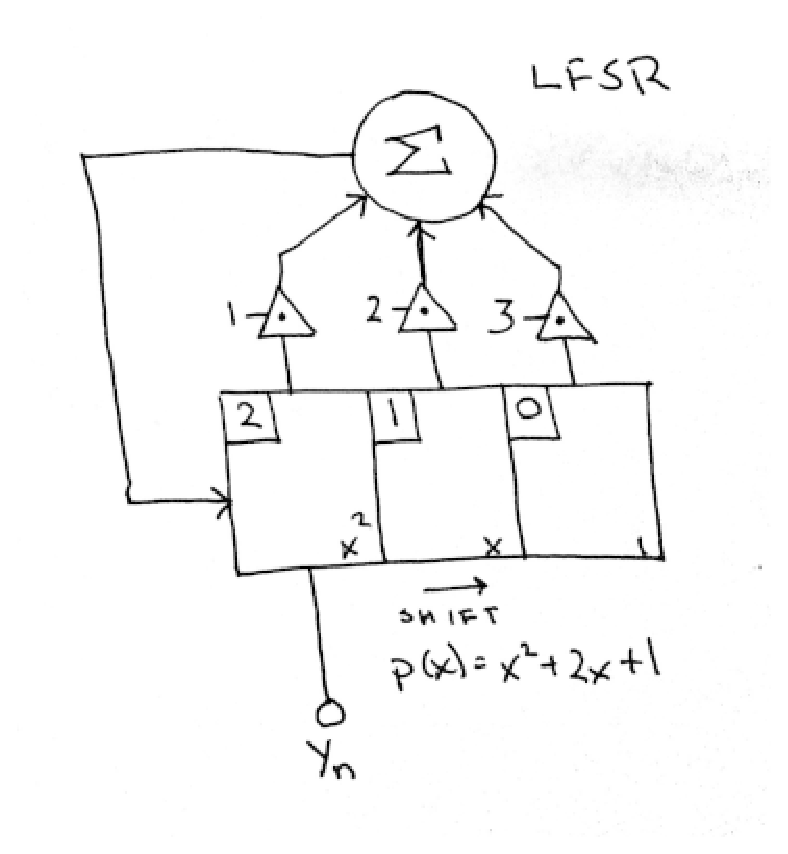
\includegraphics{./figures/lfsr-2.eps}
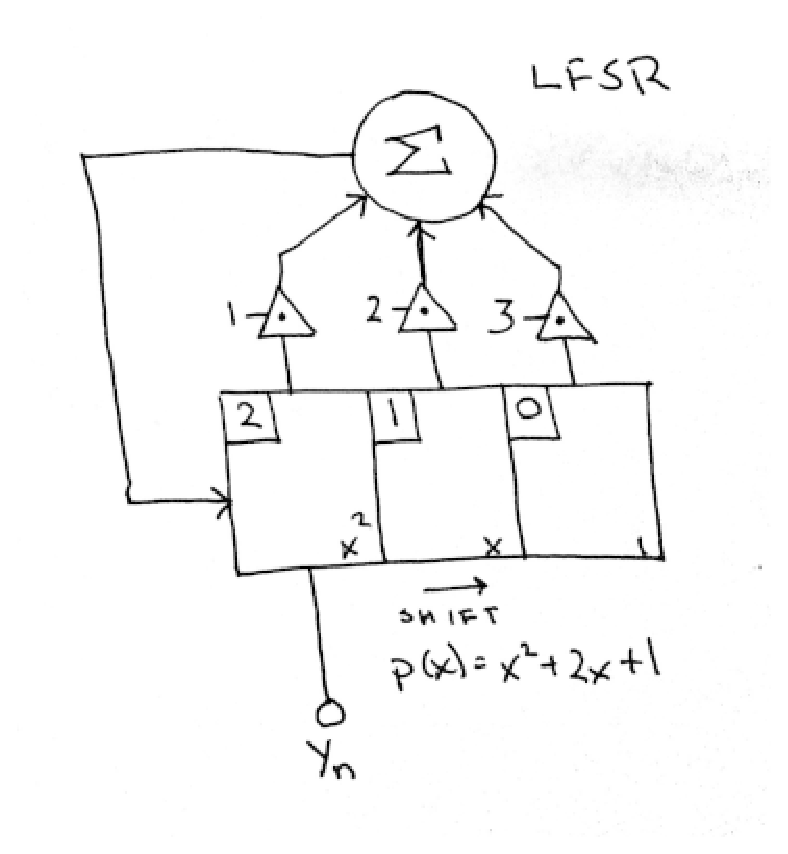
\includegraphics{./figures/lfsr-2.eps}
\end{center}
\caption{Linear Feedback Shift Register (LFSR)}
\label{fig:lfsr}
\end{figure}

State Space Representation
\newline

\begin{equation}
\mathbf{X}_k = \mathbf{F}\mathbf{X}_{k-1}
\label{eq:ss_rep}
\end{equation}

\begin{equation}
\stackrel{\mbox{$X_k$}}{
\left[ \begin{array}{c}
x^{'}_{0} \\
x^{'}_{1} \\
x^{'}_{2} \\
\end{array} \right]
}
= 
\stackrel{\mbox{$F$}}{
\left[ \begin{array}{ccc}
1 & 2 & 3 \\
1 & 0 & 0 \\
0 & 1 & 0 \\
\end{array} \right]
}
\stackrel{\mbox{$X_{k-1}$}}{
\left[ \begin{array}{c}
x_{0} \\
x_{1} \\
x_{2} \\
\end{array} \right]
}
\label{eq:ss_rep_2}
\end{equation}

where

\begin{equation}
\mathbf{X}_0 = 
\stackrel{\mbox{$X_{0}$}}{
\left[ \begin{array}{c}
2 \\
1 \\
0 \\
\end{array} \right]
}
\label{eq:ss_x0}
\end{equation}

so

\begin{equation}
\mathbf{X}_k 
= \mathbf{F}\mathbf{X}_{k-1}
= \mathbf{F} \left( \mathbf{F}\mathbf{X}_{k-2} \right)
= \mathbf{F} \left( \mathbf{F} \left( \mathbf{F}\mathbf{X}_{k-3} \right) \right)
= \cdots
= \mathbf{F}^N \mathbf{X}_0
\label{eq:ss_rep_expanded}
\end{equation}

              \schemelist{../chapter-1/sicp_ch1_e1-11.scm}
              \outlist{../output/sicp_ch1_e1-11.out}
            \subsubsection{Tree Recursion}
            \subsubsection{Orders of Growth}
            \subsubsection{Exponentiation}
              \schemelist{../chapter-1/sicp_ch1_e1-16.scm}
              \outlist{../output/sicp_ch1_e1-16.out}
            \subsubsection{Greatest Common Divisors}
            \subsubsection{Example: Testing for Primality}
        \subsection{Formulating Abstractions with Higher-Order Procedures}
            \subsubsection{Procedures as Arguments}
            \subsubsection{Constructing Procedures Using Lambda}
            \subsubsection{Procedures as General Methods}
            \subsubsection{Procedures as Returned Values}
              \schemelist{../chapter-1/sicp_ch1_e1-42.scm}
              \outlist{../output/sicp_ch1_e1-42.out}

%% *EOF*
